
\section{Extending the algebra structure}
\label{Extension}
First we define a replacement for $\sset$ which is needed when extending the multiplication.

\begin{Definition}
Let $\DLat$ be the category of finite distributive lattices. The objects of interest to us in $\DLat$ are $\aug{X}$ for $X$ a finite grid poset (see \autoref{22case}) or a disjoint union of finite grids.

Define $\lSet$ to be the category of presheaves on $\DLat$.
\end{Definition}

Our goal in this section is to extend $H_{comb}$ to a functor $\OrdSet\otimes\OrdSet\to\Corr(\lSet^{op})$ and the Waldhausen construction to a functor $\lSet^{op}\to\Spaces$. Here by $\otimes$ we mean the Gray tensor of categories. All together we get an extension of $H_{geom}$ to a functor $\OrdSet\otimes\OrdSet\to\Corr(\Spaces)$
%%%%%%%%%%%%%%%%%%%%%%%%%%%%%%%%%%%%%%%%%%%
%%%%%%%%%%%%%%%%%%%%%%%%%%%%%%%%%%%%%%%%%%%

\subsection{Extension of \texorpdfstring{$H_{comb}$}{Hcomb}}
We explain the basics of the extension which will appear in detail in \cite{GeometricHallAlgebra2}.

\subsubsection{On objects}
An object of $\OrdSet\otimes\OrdSet$ is just a pair of objects $(X,Y)$ of $\OrdSet$. We consider first the grid poset $X\times Y$, and similarly to the construction in \autoref{HcombObjects} we note that for every \emph{level set} $(X\times Y)_d$ of the grid (i.e. the vertices at distance $d$ from the origin) we have an imbedding $\aug{(X\times Y)_d}$ in $\aug{X\times Y}$ and we define $H_{comb}(X,Y)$ to be the sub-$\lSet$ generated by the images of these imbeddings.

\begin{Example}
$H_{comb}(\ord{2},\ord{2})$ corresponds to the picture
\[
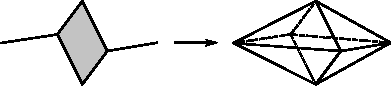
\includegraphics{Figures/squareHcombObject.pdf}
\]
\end{Example}
 where the right diagram is the poset $\aug{\ord{2}\times\ord{2}}$

\subsubsection{On arrows}
\label{HallCombArrows}
The arrows of $\OrdSet\otimes\OrdSet$ are generated by pairs of maps $(X,Y)\xrightarrow{f,g}(Z,W)$, where one of $(f,g)$ is the identity.

These generating arrows can be thought of as projections of grids. So suppose $P\xrightarrow{f} Q$ is such a projection. We want to construct a correspondence \[
\stik{1}{
H_{comb}(P) \ar{r}{s} \& X \& \ar{l}{p} H_{comb}(Q)
}
\]
We have a natural candidate for $X$: For any $d$, we consider the preimage of the level set $f^{-1}(Q_d)\subset P$, and in the same way as above we have an imbedding $\aug{f^{-1}(Q_d)}\to \aug{P}$. We let $X:=H_{comb}(f)$ be the sub-$\lSet$ generated by these images. An easy check shows that the map $\aug{Q}\xrightarrow{\aug{f}}\aug{P}$ lands in $H_{comb}(f)$ so defines the map $p$.

\textbf{Problem}: There is no natural map $H_{comb}(P)\to H_{comb}(f)$.

\textbf{Proposed solution}: We consider all intersections $f^{-1}(Q_d)\cap P_{d'}$ and the imbeddings of their augmentations in $\aug{P}$ and call what is generated $\overline{H_{comb}(f)}$. We now have a diagram\[
\stik{1}{
H_{comb}(P) \&\ar{l}{w} \overline{H_{comb}(f)} \ar{r}{s} \& H_{comb}(f) \& \ar{l}{p} H_{comb}(Q)
}
\]

\textbf{Why is this reasonable?} The maps $w$ go to an equivalence of stacks under $S$, so this can be considered as a localization.

\begin{Example}
\label{splitComb}
Consider the map $P=\ord{2}\times\ord{2}\xrightarrow{f}\ord{2}\times\ord{1}=Q$. It corresponds to the picture
\[
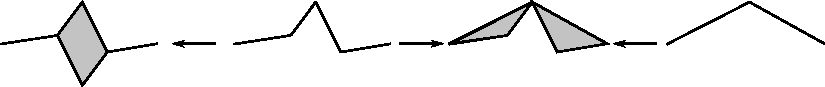
\includegraphics[scale=0.8]{Figures/squareHcombArrow.pdf}
\]
\end{Example}
In \autoref{splitWald} we explain in detail where the parts of this picture go under the extended Waldhausen construction.

\subsubsection{On squares}
\label{HCombSquares}
We start by giving the example of the square
\[
\stik{1}{
(\ord{2},\ord{2}) \ar{d}{} \ar{r}{} \& (\ord{2},\ord{1}) \ar{d}{} \\
(\ord{1},\ord{2}) \ar{r}{} \& (\ord{1},\ord{1})
}
\]
which goes to the Hopf relation.

It corresponds to the commutative diagram
\[
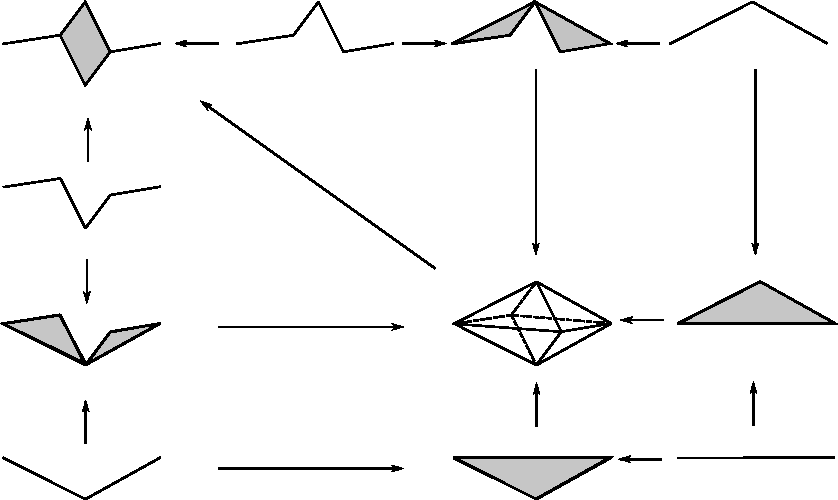
\includegraphics[scale=0.8]{Figures/HallHopfComb.pdf}
\]

From this example it should be clear how to write the image of a general square as a diagram in $\lSet$. The only issue is what kind of object this should be considered as. Our idea is that this should be considered as a square in the double category of correspondences in the localization double category of $\lSet$ at some class of "weak equivalences". We plan to explore this further in a future work.

For the purposes of this article however, all we need are constructions of certain squares and cubes and we verify the parts of the functoriality that we need locally.

%%%%%%%%%%%%%%%%%%%%%%%%%%%%%%%%%%%%%%%%%%%
%%%%%%%%%%%%%%%%%%%%%%%%%%%%%%%%%%%%%%%%%%%

\subsection{Extension of the Waldhausen construction}
\label{ExtWaldhausen}
Note that the $S$ construction from \autoref{Waldhausen} extends verbatim to the category $\POSet$ of finite posets. 

Note that also the augmentation functor extends to $\POSet\to \POSet^{op}$ by setting \[
\aug{X}=\Hom_{\POSet}(X,0\to 1)
\]

In fact all the posets that appear as augmentations in our picture are distributive lattices, so we think of $S$ as being defined on $\DLat$, and we claim that it naturally extends to $\lSet$. This depends on the behaviour of $S$ with respect to limits/colimits, along the lines of the 2-Segal property from \cite{KapranovDyckerhoff}.

\begin{Remark}
The category of presheaves on $\DLat$ appears in other contexts, for example as a framework for homotopy type theory in \cite{cubicalHott}.
\end{Remark}

%%%%%%%%%%%%%%%%%%%%%%%%%%%%%%%%%%%%%%%
%%%%%%%%%%%%%%%%%%%%%%%%%%%%%%%%%%%%%%
\subsubsection{The image of the square}
\label{22case}
Let $X=\aug{\ord{2}\times\ord{2}}$. This case plays a central role in our computation of the braiding.

%For simplicity we consider $\CCC$ to be (the $\infty$-derived category of) $\Vect$.

We start with a square
\[
\stik{1}{
1 \ar{r} \ar{d} \& 2 \ar{d}\\
3 \ar{r} \& 4
}
\]
 and consider its augmentation, i.e. all maps to $0\to 1$. If we denote by $M_T$ the map that sends the vertices in $T$ to $0$, then we see that $X$ is the poset

\[
\stik{1}{
{} \& {} \& M_{\{1,3\}}\ar{dr} \ar{drr} \& {} \& {} \\
M_{\{1,2,3,4\}} \ar{r} \ar{urr} \ar{drr} \& M_{\{1,2,3\}} \ar{ur} \ar{dr} \& {} \& M_{\{1\}} \ar{r} \& M_{\emptyset} \\
{} \& {} \& M_{\{1,2\}} \ar{ur} \ar{urr} \& {} \& {}
}
\]

Note that the top and bottom rows are the embeddings of $\aug{\ord{2}}$ coming from the projections from $\ord{2}\times\ord{2}$ to $\ord{2}$.

For the next step, recall that under Waldhausen construction the category that gets associated to \[
0\to 1 \to 2 = \aug{\ord{2}}
\]
is the category of short exact sequences
\[
0\to V_{01}\to V_{02}\to V_{12} \to 0
\]
For convenience, let us relabel the vertices of $X$ as

\begin{equation}
\label{augmentedSquare}
\stik{1}{
{} \& {} \& v\ar{dr} \ar{drr} \& {} \& {} \\
S \ar{r} \ar{urr} \ar{drr} \& 1 \ar{ur} \ar{dr} \& {} \& 2 \ar{r} \& T \\
{} \& {} \& h \ar{ur} \ar{urr} \& {} \& {}
}
\end{equation}
Then just by considering the sub-posets isomorphic to $\aug{\ord{2}}$, we see that an object of $S_X\CCC$ must contain a system of short exact sequences
\[
\nnstik{1}{
{S1} \ar{rr} \ar{dd}\& {} \& {Sv} \ar{dd} \ar{rr} \& {} \& {1v}\\
{} \& {} \&{} \& {h2} \ar{dr}\\
{Sh} \ar{rr} \ar{dd}\& {} \& {ST} \ar{dd} \ar{rr} \& {} \& {hT} \ar{dr} \\
{} \& {v2} \ar{dr} \&{} \&{} \& {} \& {2T}\\
{1h} \& {} \& {vT} \ar{dr} \& {} \& {} \\
{} \& {} \&{} \& {2T} \ar[equal]{uurr}
}
\]
(where labels $\alpha\beta$ denote the corresponding map $(0\to 1)\to X$ and colinear terms in the diagram form a short exact sequence)

Further analysing $\grid{X}$ we see that a map $\grid(X)\to \CCC$ contains pullback squares of the form
\[
\stik{1}{
0 \ar{r} \ar{d} \& 0\ar{d}\\
1v \ar{r} \& h2
}
\stik{1}{}
\stik{1}{
0 \ar{r} \ar{d} \& 0\ar{d}\\
1h \ar{r} \& v2
}
\]
 which gives us isomorphisms $1v\xrightarrow{\sim} h2$ and $v2\xrightarrow{\sim} 1h$.
 
In all we see that $S_X\CCC$ is equivalent to the category of grids
\[
\nnstik{1}{
{S1} \ar{rr} \ar{dd}\& {} \& {Sv} \ar{dd} \ar{rr} \& {} \& {1v} \ar{dd}\\
{} \& {} \&{} \& {} \\
{Sh} \ar{rr} \ar{dd}\& {} \& {ST} \ar{dd} \ar{rr} \& {} \& {hT} \ar{dd} \\
{} \& {}  \&{} \&{} \& {} \& {}\\
{1h} \ar{rr} \& {} \& {vT} \ar{rr} \& {} \& {2T}
}
\]


%%%%%%%%%%%%%%%%%%%%%%%%%%%%%%%%%%%%%%%
%%%%%%%%%%%%%%%%%%%%%%%%%%%%%%%%%%%%%%

\subsubsection{\autoref{splitComb} revisited}
\label{splitWald}

We now explain what the extended Waldhausen construction does to the diagram 
\[
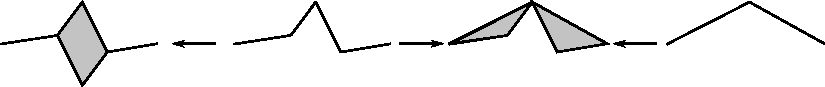
\includegraphics[scale=0.8]{Figures/squareHcombArrow.pdf}
\]

The three rightmost objects correspond to the picture
\[
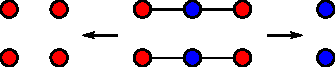
\includegraphics{Figures/HallHopfDoubleMult.pdf}
\]

Let us now consider the leftmost object and write it as a union of lattices, using the notation in \autoref{augmentedSquare}
\[
\stik{1}{
{} \& {} \& v\ar{dr} \& {} \& {} \\
S \ar{r}   \& 1 \ar{ur} \ar{dr} \& {} \& 2 \ar{r} \& T \\
{} \& {} \& h \ar{ur}  \& {} \& {}
}
\]

Repeating the relevant parts of the computation following \autoref{augmentedSquare}, we see that the Waldhausen construction sends this to the stack consisting of triples:
\begin{itemize}
    \item An object $S1$
    \item An object $2T$
    \item A diagram
    \[
    \nnstik{1}{
{}  \& {} \& {1v} \ar{dd} \ar{ddrr}[above,sloped]{\sim} \& {} \& {} \\
{} \& {} \&{} \& {} \\
{1h} \ar{rr} \ar{ddrr}[above,sloped]{\sim} \& {} \& {12} \ar{dd} \ar{rr} \& {} \& {h2}  \\
{} \& {}  \&{} \&{} \& {} \& {}\\
{}  \& {} \& {v2} \& {} \& {}
}
    \]
    where the row and column are short exact sequences
\end{itemize}

The leftmost map is then just the assignment to the quadruple of objects $(S1,1v,v2,2T)$ which can easily be seen to be an equivalence.

